% THIS IS SIGPROC-SP.TEX - VERSION 2.9
% WORKS WITH V3.0SP OF ACM_PROC_ARTICLE-SP.CLS
% MARCH 2007
%
% It is an example file showing how to use the 'acm_proc_article-sp.cls' V3.0SP
% LaTeX2e document class file for Conference Proceedings submissions.
% ----------------------------------------------------------------------------------------------------------------
% This .tex file (and associated .cls V3.0SP) *DOES NOT* produce:
%       1) The Permission Statement
%       2) The Conference (location) Info information
%       3) The Copyright Line with ACM data
%       4) Page numbering
% ---------------------------------------------------------------------------------------------------------------
% It is an example which *does* use the .bib file (from which the .bbl file
% is produced).
% REMEMBER HOWEVER: After having produced the .bbl file,
% and prior to final submission,
% you need to 'insert'  your .bbl file into your source .tex file so as to provide
% ONE 'self-contained' source file.
%
% Questions regarding SIGS should be sent to
% Adrienne Griscti ---> griscti@acm.org
%
% Questions/suggestions regarding the guidelines, .tex and .cls files, etc. to
% Gerald Murray ---> murray@acm.org
%
% For tracking purposes - this is V2.9SP - MARCH 2007

\documentclass{acm_proc_article-sp}
 
\usepackage{color}

%-- Begin patch area for accents in 'Author Block' area - may be needed by some authors / but not all
\DeclareFixedFont{\auacc}{OT1}{phv}{m}{n}{12}   % Needed for "Author Block" accents - Patch by Gerry 3/21/07
\DeclareFixedFont{\afacc}{OT1}{phv}{m}{n}{10}   % Needed for "Author Block" accents in the affiliation/address line - Patch by Gerry 3/21/07
%--
\begin{document}

\title{COMP6006: Intelligent Agents Report}
 \subtitle{The BeadyEye Agent
%\titlenote{A full version of this paper is available as
%\textit{Author's Guide to Preparing ACM SIG Proceedings Using
%\LaTeX$2_\epsilon$\ and BibTeX} at \texttt{www.acm.org/eaddress.htm}}
}
%
% You need the command \numberofauthors to handle the 'placement
% and alignment' of the authors beneath the title.
%
% For aesthetic reasons, we recommend 'three authors at a time'
% i.e. three 'name/affiliation blocks' be placed beneath the title.
%
% NOTE: You are NOT restricted in how many 'rows' of
% "name/affiliations" may appear. We just ask that you restrict
% the number of 'columns' to three.
%
% Because of the available 'opening page real-estate'
% we ask you to refrain from putting more than six authors
% (two rows with three columns) beneath the article title.
% More than six makes the first-page appear very cluttered indeed.
%
% Use the \alignauthor commands to handle the names
% and affiliations for an 'aesthetic maximum' of six authors.
% Add names, affiliations, addresses for
% the seventh etc. author(s) as the argument for the
% \additionalauthors command.
% These 'additional authors' will be output/set for you
% without further effort on your part as the last section in
% the body of your article BEFORE References or any Appendices.

\numberofauthors{1} %  in this sample file, there are a *total*
% of EIGHT authors. SIX appear on the 'first-page' (for formatting
% reasons) and the remaining two appear in the \additionalauthors section.
%
\author{
% You can go ahead and credit any number of authors here,
% e.g. one 'row of three' or two rows (consisting of one row of three
% and a second row of one, two or three).
%
% The command \alignauthor (no curly braces needed) should
% precede each author name, affiliation/snail-mail address and
% e-mail address. Additionally, tag each line of
% affiliation/address with \affaddr, and tag the
% e-mail address with \email.
%
% 1st. author
\alignauthor
Rikki Prince\\
       \affaddr{University of Southampton}\\
       \affaddr{Highfield}\\
       \affaddr{Southampton, UK}\\
       \email{rfp102@soton.ac.uk}
}
% There's nothing stopping you putting the seventh, eighth, etc.
% author on the opening page (as the 'third row') but we ask,
% for aesthetic reasons that you place these 'additional authors'
% in the \additional authors block, viz.
%\additionalauthors{Additional authors: John Smith (The Th{\o}rv\"{a}ld Group,
%email: {\texttt{jsmith@affiliation.org}}) and Julius P.~Kumquat
%(The Kumquat Consortium, email: {\texttt{jpkumquat@consortium.net}}).}
\date{}
% Just remember to make sure that the TOTAL number of authors
% is the number that will appear on the first page PLUS the
% number that will appear in the \additionalauthors section.

\maketitle

\pagenumbering{arabic}

\begin{abstract}
 %%%%%%%%%%%%
 % ABSTRACT %
 %%%%%%%%%%%%
 \textcolor{red}{FILL THIS IN.}
\end{abstract}

% A category with the (minimum) three required fields
%\category{H.4}{Information Systems Applications}{Miscellaneous}
%A category including the fourth, optional field follows...
%\category{D.2.8}{Software Engineering}{Metrics}[complexity measures, performance measures]

%\terms{Delphi theory}

%\keywords{ACM proceedings, \LaTeX, text tagging} % NOT required for Proceedings

\section{Introduction}
 \label{intro}

 This report describes the approach taken in creating a software agent to compete in a TAC Classic contest hosted at the University of Southampton for the module COMP6006: Intelligent Agents.
 
 This introduction further explains the format of the competition.  Then Section~\ref{approach} discusses overall approach taken by this agent, Section~\ref{design} describes the design used to implement this approach and Section~\ref{heuristics} explains some of the heuristics used to make bidding decisions.  Section~\ref{res} presents the results of the competition, after which Section~\ref{eval} evaluates this agent's performance.  Finally, some future improvements are suggested in Section~\ref{future}, before conclusions are drawn in Section~\ref{conc}.
 
 \subsection{TAC}
 The Trading Agent Competition (TAC) is an annual contest organised by, and for, the agent research community, with the assistance of the Swedish Institute of Computer Science (SICS) since 2002.  The hope is that by fostering a competetive spirit, the advancement of the field will be accelerated.  The competition current consists of two scenarios: TAC Classic and TAC SCM \cite{SICS2007a}.
 
 It is the TAC Classic scenario which was faced in this challenge.  This scenario involves acting as a ``travel agent", to create holiday packages to suit the requirements of a group of eight customers.  A holiday package consists of inbound and outbound flights, a hotel room for each night of the stay and tickets to entertainment venues.  Further complexity is added by the fact that there are two hotels to choose from and three entertainment venues.  In total, the agent is required to co-ordinate bidding strategies in up to 28 different auctions.
 
 The auctions also vary in format.  The flight auctions clear instantly, but have a sell price which varies every 10 seconds, based on a stochastic function.  An auction is held for each night, in each hotel, though only 16 rooms are available per hotel.  Therefore the auction is an ascending-price, multi-unit English auction, where the 16 winners pay the 16th highest price.  The quirk is that one hotel auction closes every minute, in a randomly selected order.  Finally, entertainment auctions allow agents to buy and sell tickets from each other once they negotiate a price \cite{SICS2007b}.
 
 Bidding in auctions is performed by sending bid strings to the TAC server, containing the number of items required and the price the agent is willing to pay.  Fortunately, the process of submitting bids and retrieving information about the clients' preferences and current state of the auctions is made slightly easier by the TAC Classic Java Agent Ware \cite{SICS2007c}.
 
 At the end of a TAC game, the competing agents are ranked against each other based on how well they fulfilled their clients' requirements.  The measure of fulfillment is known as the utility, and is based upon how close the package is to the clients' preferred start and end dates, as well as whether the package matches the quality of hotel the client wanted and includes their favoured entertainment.  The final score for the agent is the total utility, minus the costs of purchasing the various items which make up the packages.
 
 \subsection{The COMP6006 Contest}
 
 The contest held for the COMP6006 module ran over two days.  Entrants competed on one of the two days, against up to 25 others.  However, as each game only allows for eight competitors at a time, the two days were arranged so that each agent would compete in around 10-15 games, against a different group of opponents in each game.
 
 To vary the level of the competition, and provide somewhat of a benchmark, the agent which finished second in the 2005 actual TAC contest, ``Dolphin", and the DummyAgent provided in the Agent Ware, were both included as competitors.
 
\section{Approach}
 \label{approach}

 The initial aproach taken was to better encapsulate the data available into Java objects, so that programming the decision making aspects of the code would be more intuitive to write and manipulate.  Agent Ware provides access to client preferences with lines of code such as:
 \begin{verbatim}
  agent.getClientPreference(c, TACAgent.ARRIVAL);
 \end{verbatim}
 Once the agent logic becomes more complex, calling this line of code just to find a client's preferred arrival day could make the code complicated to read.  The intended alternative is to create an object for each client, which provides a method for requesting the arrival day, as well as all other preferences, for example:
 \begin{verbatim}
  client[c].start();
 \end{verbatim}
 The added advantage of this approach is that certain decisions and calculations can be performed within the confines of the object, rather than in some arbitrary place within the agent.  For instance, one of the important tasks that can be processed within the client object is to allocate hotel rooms, flights and entertainment tickets that have been won, and therefore provisionally calculate the utility and cost of a particular client's package.
 
 As well as the client, other concepts within the TAC contest that can be compartmentalised into an object are the flight, hotel and entertainment auctions.
 
 Within the agent, the flow of activity expected to occur is as follows:
 \begin{enumerate}
  \item Allocate initial entertainment to clients if they require them.
  \item Submit initial bids for hotel rooms.
  \item Upon a transaction, allocate item won to client that requires it.
   \begin{itemize}
    \item If client has all the hotel rooms it needs, purchase flights.
    \item If client has both inbound and outbound flights, purchase suitable entertainment.
   \end{itemize}
 \end{enumerate}

\section{Design}
 \label{design}

 As discussed above, the approach taken was to construct objects for storing the available data in a more logical format.  This section describes the design of the classes that store and process this data.  These classes work on top of the Agent Ware code, the design of which is not examined here.
 
 \subsection{Client}
  The primary abstraction from the data provided by the Agent Ware is that of the client.  The client is the main focus of the agent's efforts, so it makes sense to encapsulate some of the decision-making functionality of the agent within a client object.
  
  Within this agent, the Client had to be designed to store both the original client preferences, and any updated preferences that result from changes within the game environment.  Once a hotel auction closes, if the agent did not win the required number of rooms for that night, the client's preferred package could become invalid, and hence the requirements of that client would have to change.  Additionally, the Client must keep track of any rooms, flights or entertainment tickets which have been allocated to it, and how much they cost to purchase.
  
\begin{figure}
  \begin{center}
    %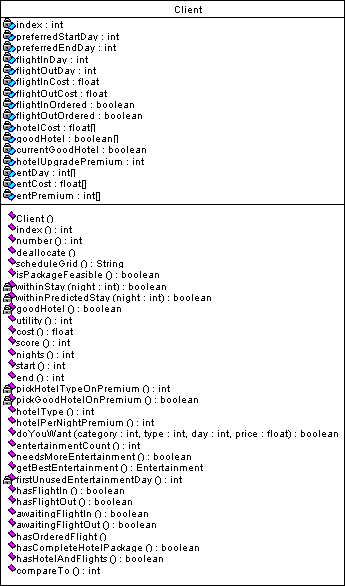
\includegraphics[keepaspectratio=true, width=10cm]{client2}
    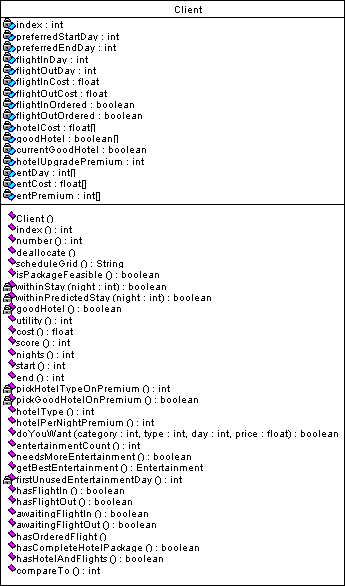
\includegraphics[keepaspectratio=true, width=0.35\textwidth]{client2}
  \end{center}
  \caption{A UML class diagram depicting the Client design.}
  \label{client}
\end{figure}
  
  \subsection{Flights}
   The Flights class provides a central place for recording and analysing the flight prices, and hence deciding the best time pruchase the required flights.  As and when a client chooses a definitive day they wish to fly in or out on, the .pleaseBuy() of the Flights object is called to specify the need of a particular flight.  Every time the quote in a flight auction is updated (every 10 seconds), this information is relayed to the Flights object, which records the quote price for trend analysis both in the agent during the game, and in external statistics packages at a later date.  The analysis of the trend when the quote is updated can also trigger a bid for the flight, if the price is determined to be optimal.
   
  \subsection{Supporting Classes}
   As the standard logging used in the Agent Ware outputs to XML and is difficult to analyse, a supporting class called ``ScreenAndFile" was created to allow one method to be called to print to the standard output and to a file (the name of which is specified in the construtor).  It is also quicker to type \begin{verbatim}  OUT.println("Hello, world!");\end{verbatim} than \begin{verbatim}  System.out.println("Hello, world!");\end{verbatim}
   
   A class of static values was also created to store any common constant values that were shared by the various other classes, such as \verb"Constants.FIRST_DAY" and \verb"Constants.NUM_CLIENTS".

\section{Heuristics}
 \label{heurisitics}
 \subsection{Initial Hotel Bids}
  The main heuristic used was to determine the price to bid for hotel rooms.  Firstly, a constant is chosen to determine the total available to spend on hotel rooms over the course of the holiday.  This was initially selected to be 1000, simply based on this being the utility available for putting together a feasible package.
  
  This value then has to be split over the number of the days the client wishes to stay.  For a one night stay, this is simple, as the full amount is used.  For two nights, the value was split evenly, as if only one night was won, it does not matter which.  While the same could be done for three and four night stays, splitting the price between so many nights might reduce the likelihood of winning any hotel rooms at all for the client.  Instead, it was decided that a heavier weighting should be placed on one day, and the other nights weighted toward that night accordingly, to improve the odds of winning hotel rooms for consecutive nights.  Therefore, the hotel bid prices ratios for a three night and four night are 50\%:35\%:15\% and 40\%:30\%:20\%:10\%, respectively.
  
  Finally, if the client wishes to stay in the better TampaTowers hotel, the bid price per night is increased by the premium the client is willing to pay for the upgrade, again divided by the number of nights.
  
 \subsection{Flight Bids}
  The Flights class was designed so that analysis of the flight quotes so far could performed, and hence an optimal time to bid be calculated.  Unfortunately, there was not enough time to implement the trend analysis, so the simple heuristic of purchasing flights as soon as the client has all the hotel rooms they require, was implemented.  The reason behind this was that it avoids the risk of the flight price becoming higher.  Obviously, it does not take advantage of the fact that the price could reduce, though hopefully the price will average out over the course of a number of games.
  
 \subsection{Entertainment}
  Little was done to intelligently bid for entertainment tickets.  Once the initially owned entertainment tickets were allocated to clients, any left over were immediately placed for sale at an arbitrarily chosen price of 80.  This is a not-overly expensive price, so the ticket should eventually sell, ensuring the entertainment ticket is not wasted.
  
  When a particular Client receives all of the hotel rooms and flights they require for a feasible package, the agent elicits which entertainment would be best to purchase from the Client.  The selection process is based on whether the Client has any spare nights to visit an entertainment venue (if all nights are occupied, no entertainment is required), and then which entertainment would gain the highest utility for the Client.  The agent then simply bids the value of the utility premium, hoping that another agent is selling a ticket for less than that value, but also well aware that it will not purchase entertainment for a price higher than it will recoup in utility, so will no receive a negative score (at least in terms of entertainment).
  
  Finally, it was noticed during testing that a bug in some agents' code would cause them to bid very large amounts to purchase entertainment tickets.  As the penalty for selling an unowned ticket is only 200, it was decided that if any agent bids more than 200 for an entertainment ticket, it should be sold to them for whatever price they wish to pay for it.  Whilst slightly underhand, and rather unlikely to happen in a competition, it causes little harm to leave the code in to take advantage of such bugs.

\section{Results}
 \label{res}
 The agent describe in this report finished 17th out of twenty-three competitors on the day it competed.  If the results of the second day of competition are included, the agent ranks at 28th out of forty-eight, though this may not be a fair comparison as it did not play any TAC games against the competitors of the second day.
 
 \begin{table}		%[htbp]
 \begin{center}
%  \centering
  \begin{tabular*}{0.45\textwidth}{@{\extracolsep{\fill}} c  r  r  r }
   \hline \\
   Game No. & Utility & Cost & Score \\
   \\ \hline \\
   581 & 8766 & 5576.15 & 3189.85 \\
   584 & 8878 & 7729.70 & 1148.30 \\
   586 & 9242 & 5178.00 & 4064.00 \\
   591 & 8908 & 6239.86 & 2668.14 \\
   598 & 9500 & 6825.73 & 2674.27 \\
   599 & 0 & -28.96	& 28.97 \\
   601 & 9450 & 5206.53 & 4243.47 \\
   604 & 0 & -159.99	& 160.00 \\
   608 & 9317 & 7053.23 & 2263.77 \\
   609 & 9230 & 8635.52 & 594.48 \\ \\
   \hline \\
   Average & 7329.10 & 5225.58 & 2103.53 \\ \\
   \hline
  \end{tabular*}
 \end{center}
  \caption{Results of the 10 games played during the competition.}
  \label{results}
 \end{table}
 
 %It appears from the results in Table~\ref{results} that Games 599 and 604 were anomolous to the rest of the data, given that the utility was zero.
 
 The resulting utilities, costs and scores for each game played by this agent during the contest can be seen in Table~\ref{results}.  However, it is immediately noticeable that Games 599 and 604 produced zero utility and a negative cost, which is anomalous to the rest of the results, so most likely indicates that the agent failed to function properly.  If these results are ignored, the averages over the remaining eight games can be seen in Table~\ref{res_anom}.
 
 \begin{table}		%[htbp]
 \begin{center}
%  \centering
  \begin{tabular*}{0.45\textwidth}{@{\extracolsep{\fill}} c  r  r  r }
   \hline \\
    & Utility & Cost & Score \\
   \\ \hline \\
   Average & 9161.38 & 6555.59 & 2605.79 \\ \\
   \hline
  \end{tabular*}
 \end{center}
  \caption{Averages of the 8 consistent games.}
  \label{res_anom}
 \end{table}
 
 To add some perspective to these values, it is worth considering the averages of another agent that competed on the same day.  For this purpose, the scores of the agent supplied by the University of Southampton TAC team, Dolphin, and the top two student agents were selected, and can be seen in Table~\ref{top3}.
 
 \begin{table}		%[htbp]
 \begin{center}
%  \centering
  \begin{tabular*}{0.45\textwidth}{@{\extracolsep{\fill}} c  r  r  r }
   \hline \\
   Agent & Utility & Cost & Score \\
   \\ \hline \\
   Dolphin & 9717.7 & 5124.62 & 4593.08 \\
   tml203 & 9715 & 5485.25 & 4229.75 \\
   cjl203 & 9848.1 & 6200.25 & 3647.85 \\ \\
   \hline
  \end{tabular*}
 \end{center}
  \caption{Averages of the top 3 agents.}
  \label{top3}
 \end{table}
 
\section{Evaluation}
 \label{eval}
 Comparing the scores of the agent (disregarding the anomolous results) in Table~\ref{res_anom} with those of the top 3 agents in the competition (Table~\ref{top3}) gives a clue as to why this agent did not perform as well as others.  Firstly, the average utility gained was not as high, falling some 600 short of the better agents.  More importantly, however, the costs were significantly higher than the top two agents.

 Analysis of the log files showed that the anomalous results in Games 599 and 604 were the result of a bug in the code.  This bug resulted in Java throwing a NullPointerException, which essentially stopped the rest of the code from functioning properly.  This is why no hotel rooms or flights were purchased, and consequently why the utility was zero.  The bug occurs when the agent attempts to purchase more entertainment tickets.  If the client can choose no suitable entertainment event that it needs, the method getBestEntertainment() returns null.  The code which invokes this method fails to check whether the returned object is null before attempting to use it.
 
 The relatively consistent utility (varying from the mean by only around 4\%) over the 8 other games indicates that the clients' packages were being fairly successfully created according to their preferences.  This makes sense, as the agent only purchases flights once the hotel package has been completed, and the agent bids quite high amounts for hotels.  However, the larger disparity in the costs (up to 30\% different from the mean) suggests the purchasing strategy was somewhat flawed. In particular, savings could have been made in the purchasing of flights had some form of trend analysis been implemented, while the heuristics used to choose hotel and entertainment bid prices would have benefitted from some fine tuning.
 
\section{Future Improvements}
 \label{future}
 There are a number of tactics which this agent provides a base for, and were planned in the development of this agent but were not implemented in time for the competition.
 
 The Flights class is clearly designed so that the Client can request flights, and the Flight class will handle the responsibility of deciding when the optimal time to bid is and what is likely to be the cheapest price.  As this was not implemented, there is scope for a method to be added to calculate whether the flight price is increasing or decreasing, possibly using least squares regression \cite{Vytelingum2007}.
 
 In a similar manner to the Flights class, an EntertainmentBuyer class could be built that takes requests for certain tickets and trades to try to obtain that ticket.  The strategy could involve providing a maximum price, and the EntertainmentBuyer could bid at lower prices, slowly incrementing as time goes on, until it bids at or just under the maximum to secure the ticket in the last few minutes.  It could also recognise a required ticket for sale at a reasonable price and purchase it, and handle the buying of cheap tickets for sale at higher prices, to make a profit.
 
 A strategy that involved purchasing any hotel room that was available at a low price (such as under 10) was tested during development.  Unfortunately, it clashed with the agent's other functionality at that point in time (as hotel purchases directly triggered flight bids), so was temporarily removed.  It would certainly be possible to add this strategy to the current code, and would increase the agent's flexibility, as it would gather a pool of cheap hotel rooms to allocate to clients in case those clients' packages become infeasible.  As the hotels being purchased are extremely cheap, even if they are not used, their cost does not have too much impact on the final score.
 
 In the current code, the Client does not react to the closure of auctions.  It would improve the agent if the Client were notified when hotel auctions closed, so it could change its preferences if the package it was trying to create had become infeasible.  However, care would have to be taken to ensure the Client was notified of the auction closure \em after \em all transactions from that auction had been processed, and allocated to the appropriate Clients.
  
 One slight drawback of the Client design is that the agent can only offer it one item at a time, so allocation is essentially based on the order in which items are won.  Although this suits the current functionality of the agent, which allocates items as soon as a transaction occurs, an interesting alternative would be to store all owned flights, hotel rooms and entertainment tickets, and allow the client to choose which ones suit it best, rather than just deciding whether a particular item is suitable or not suitable.
 
 Another situation where allowing the Client to choose from all available items would be beneficial is when reallocating items.  As the allocation algorithm is essentially a greedy one, it will most likely be less than optimal.  An improvement would be to deallocate all items from the Clients and reallocate them, to allow the Clients to select better suited items.
 
 Finally, the way the Client is designed opens up an extremely interesting possibility.  With a few adjustments, the Client could be made abstract, allowing a number of Clients with different strategies.  The type of Client used could either be chosen based on the initial preferences, or chosen at random.  Essentially, each Client would be modelled as an agent, working within the confines of the main agent, so could produce some fascinating emergent properties.

\section{Conclusions}
 \label{conc}
 \textcolor{red}{FILL THIS IN.}
%\end{document}  % This is where a 'short' article might terminate

%ACKNOWLEDGMENTS are optional
\section{Acknowledgments}
 \textcolor{red}{FILL THIS IN.}
PV for help.

%
% The following two commands are all you need in the
% initial runs of your .tex file to
% produce the bibliography for the citations in your paper.
\bibliographystyle{abbrv}
%\bibliography{sigproc}  % sigproc.bib is the name of the Bibliography in this case
% You must have a proper ".bib" file
%  and remember to run:
% latex bibtex latex latex
% to resolve all references
%
% ACM needs 'a single self-contained file'!
%
\balancecolumns
% That's all folks!
\end{document}
